\begin{figure}[tbh]
    \centering
    %\subfloat[w/o gaze-adaptive stereo]{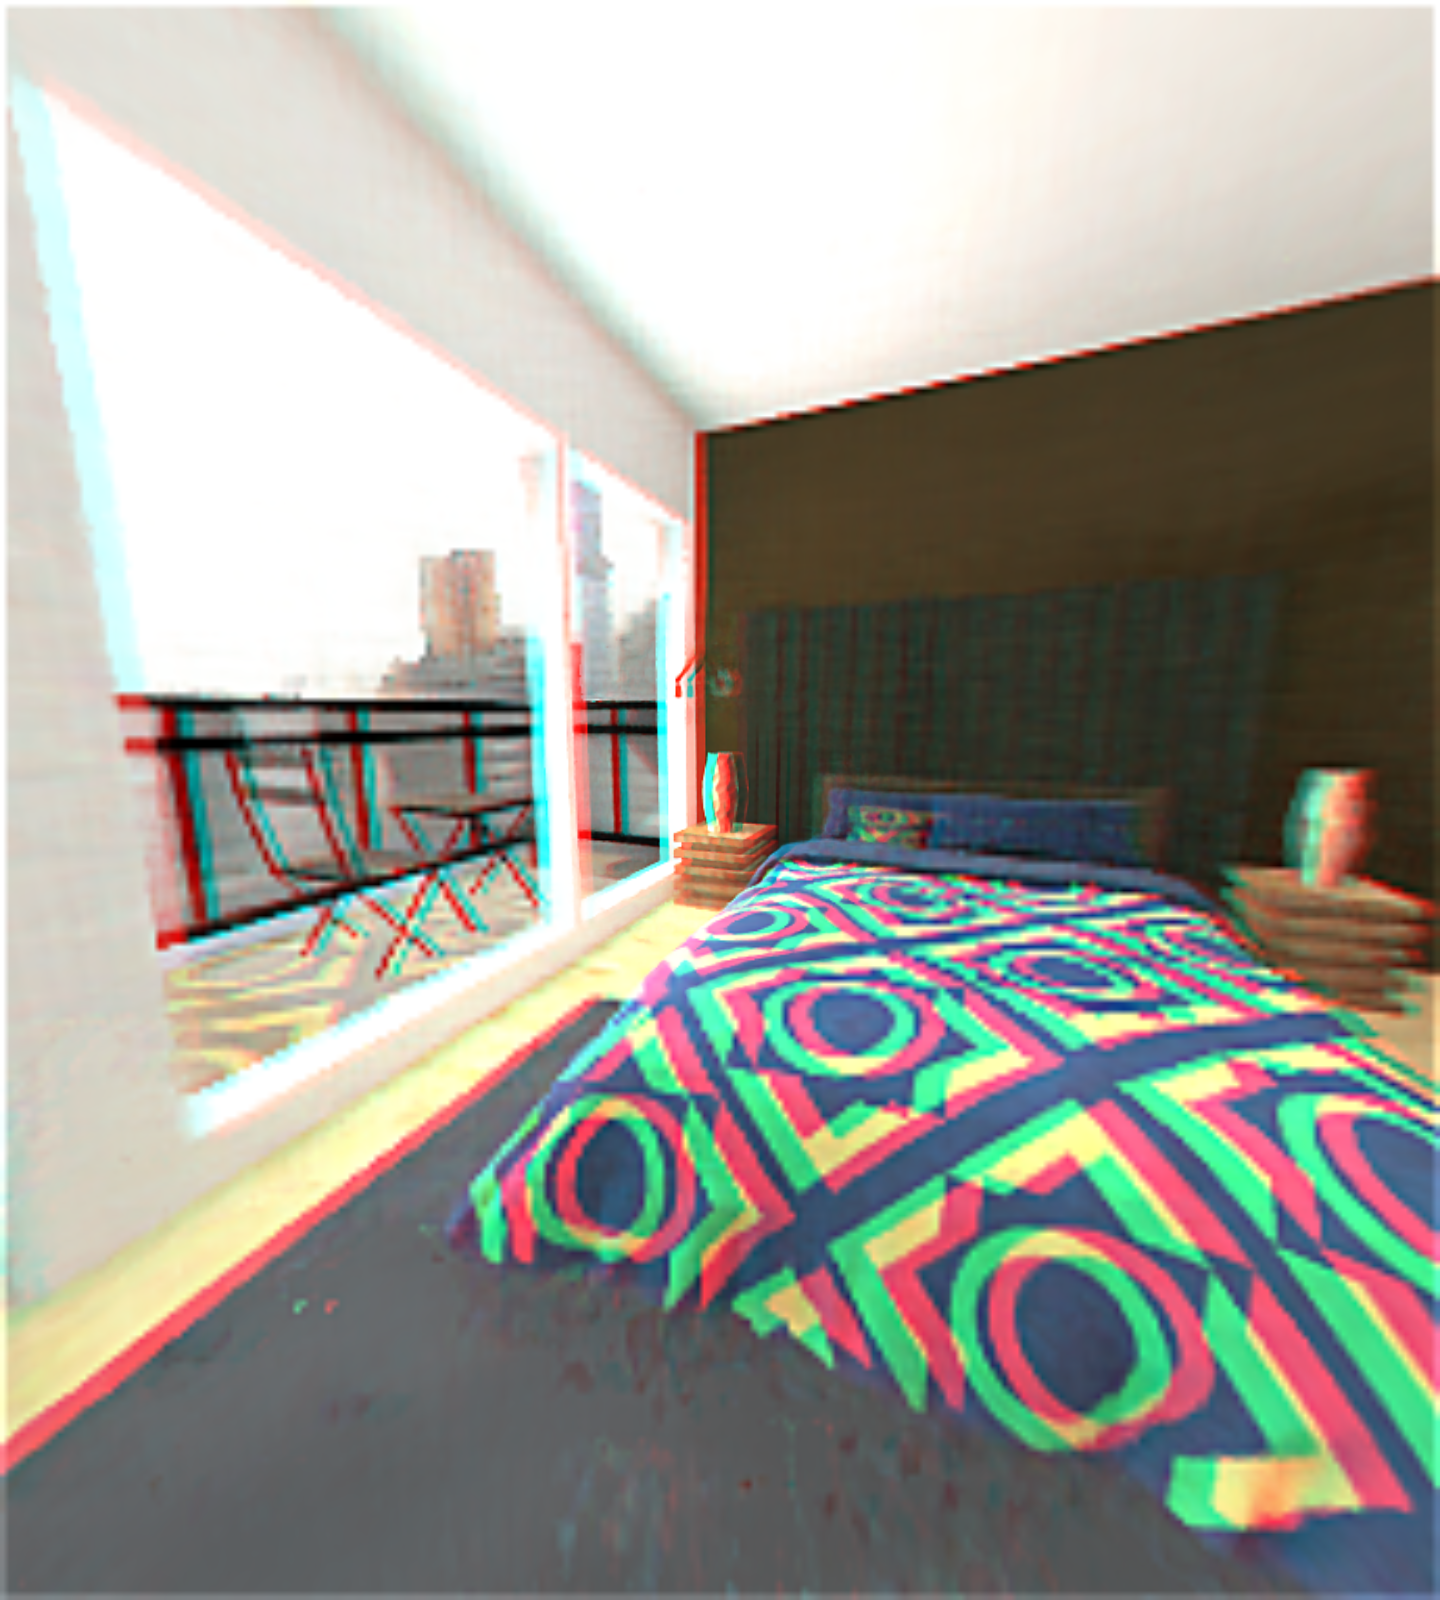
\includegraphics[width=0.248\linewidth]{TOG/figs/stereo_periphery/bedroom_view0000_blended_stereo.png}\label{fig:mono:wo}}
    %\subfloat[w/ gaze-adaptive stereo]{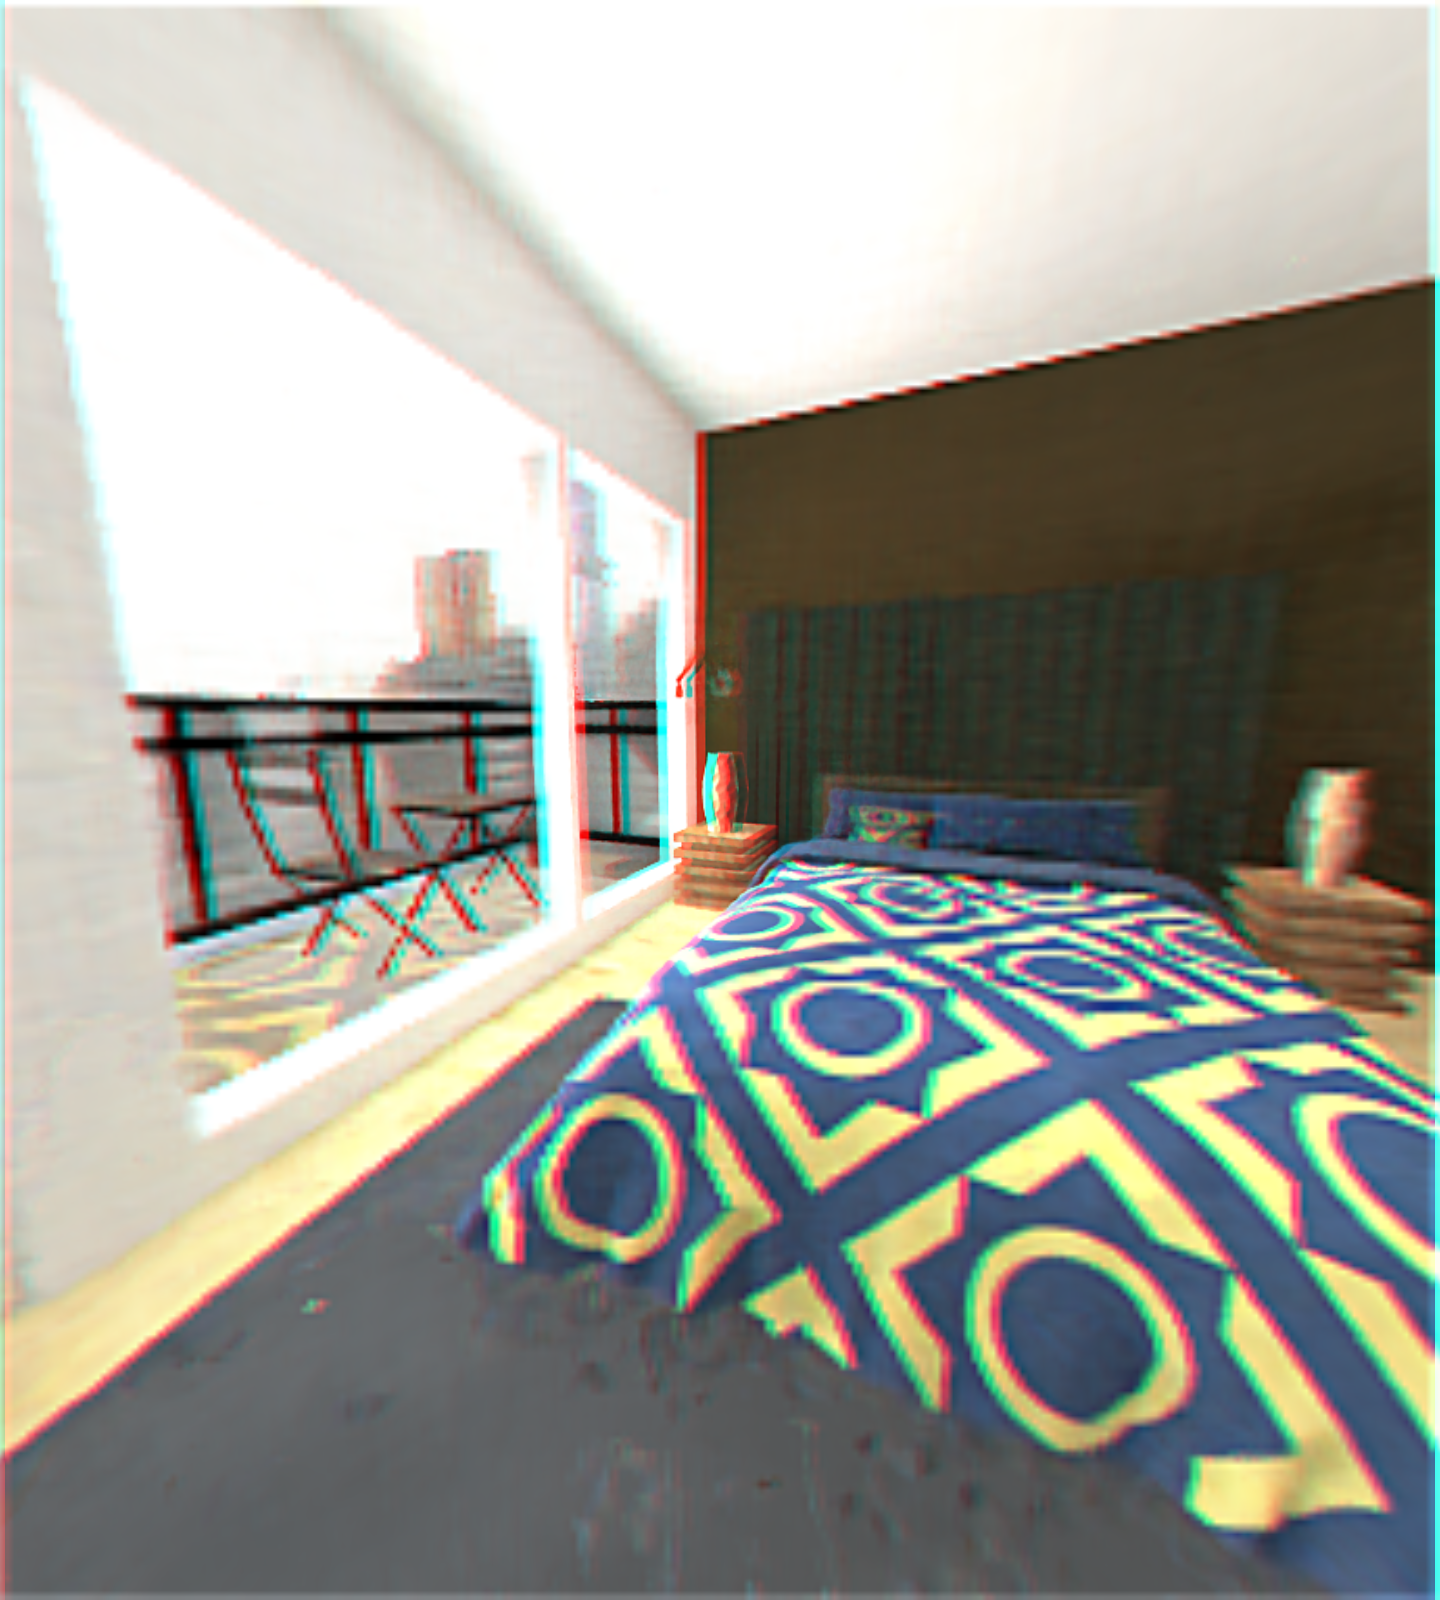
\includegraphics[width=0.248\linewidth]{TOG/figs/mono_periphery/bedroom_view0000_blended_stereo.png}%\label{fig:mono:w}}
    %\subfloat[w/o gaze-adaptive stereo]{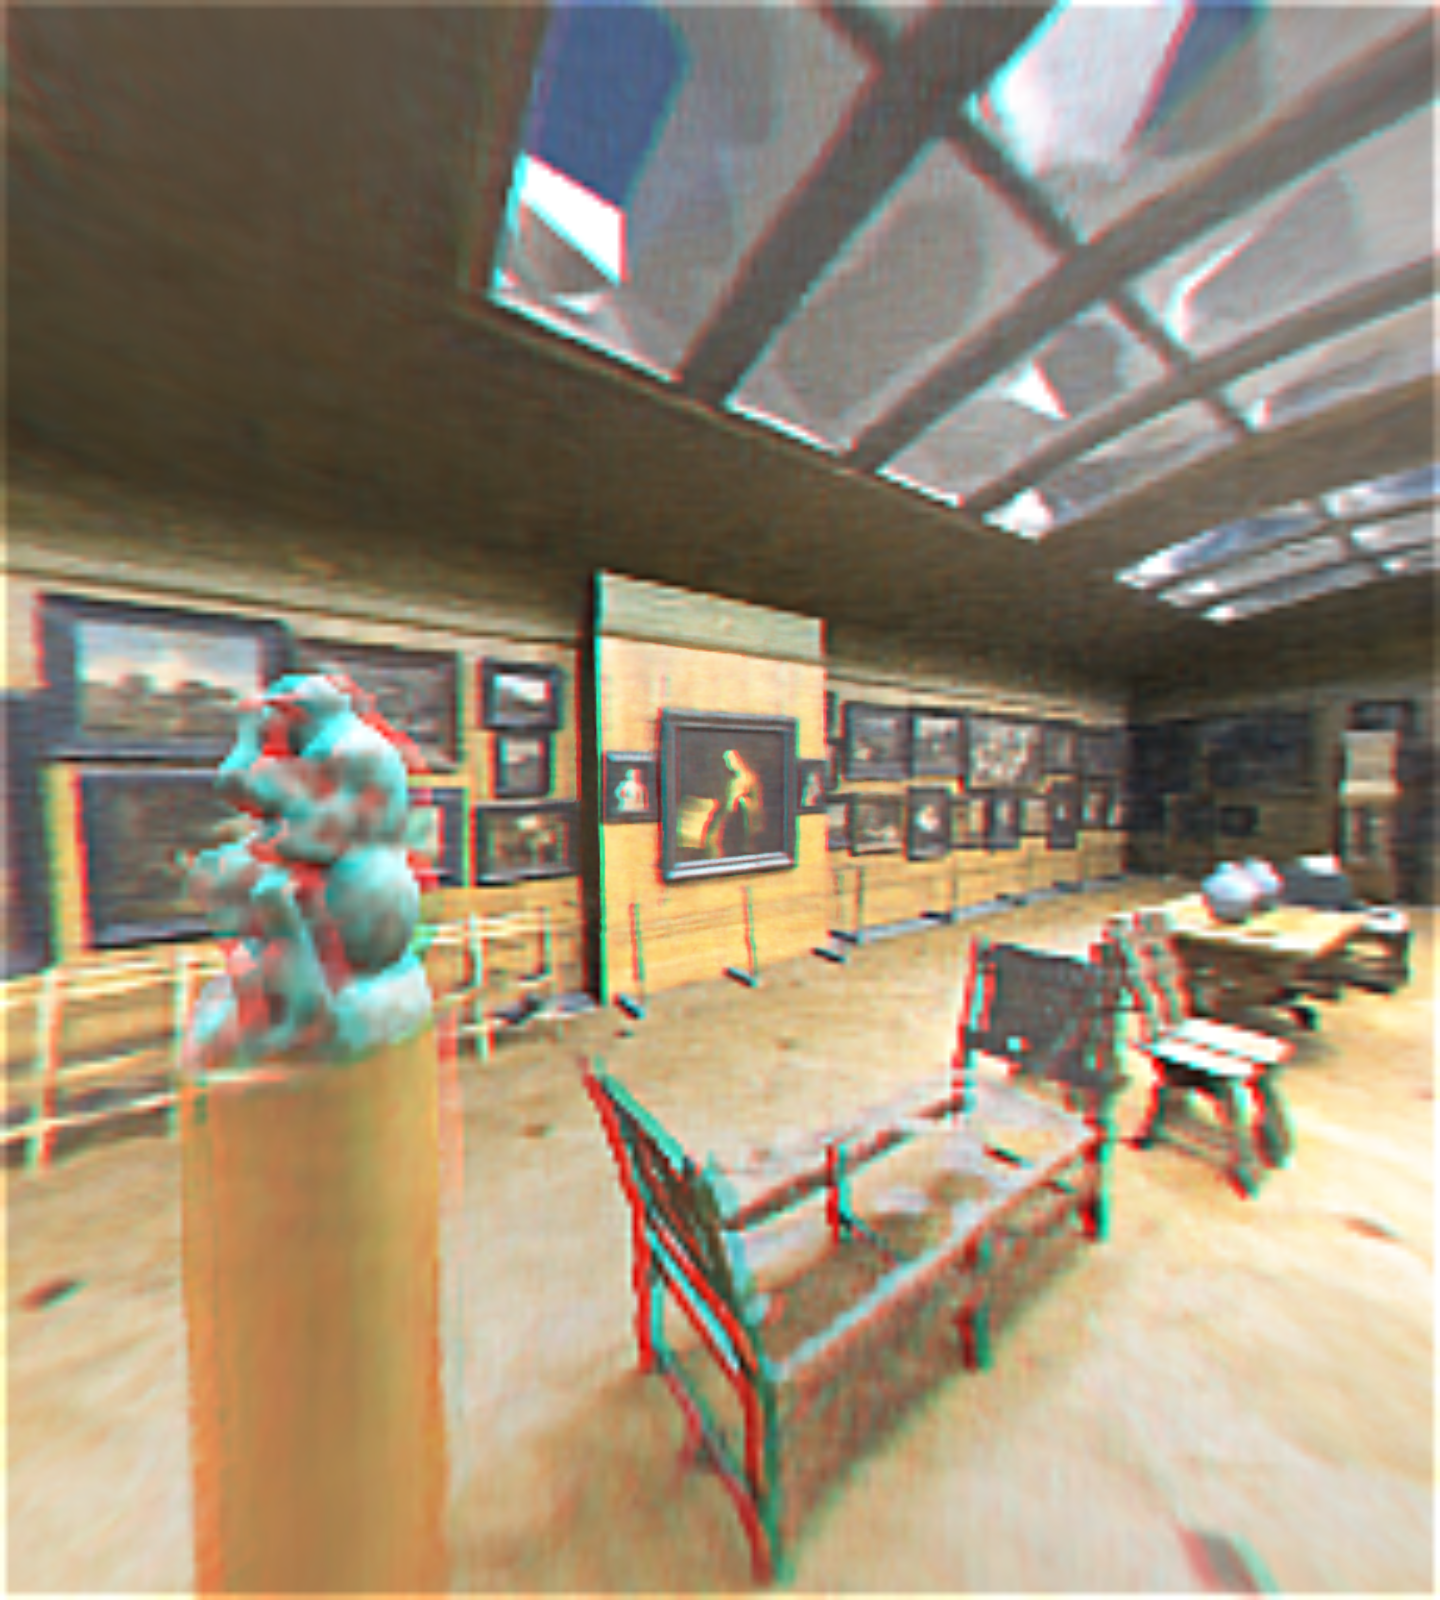
\includegraphics[width=0.248\linewidth]{TOG/figs/stereo_periphery/gallery_view0000_blended_stereo.png}\label{fig:mono:wo}}
    %\subfloat[w/ gaze-adaptive stereo]{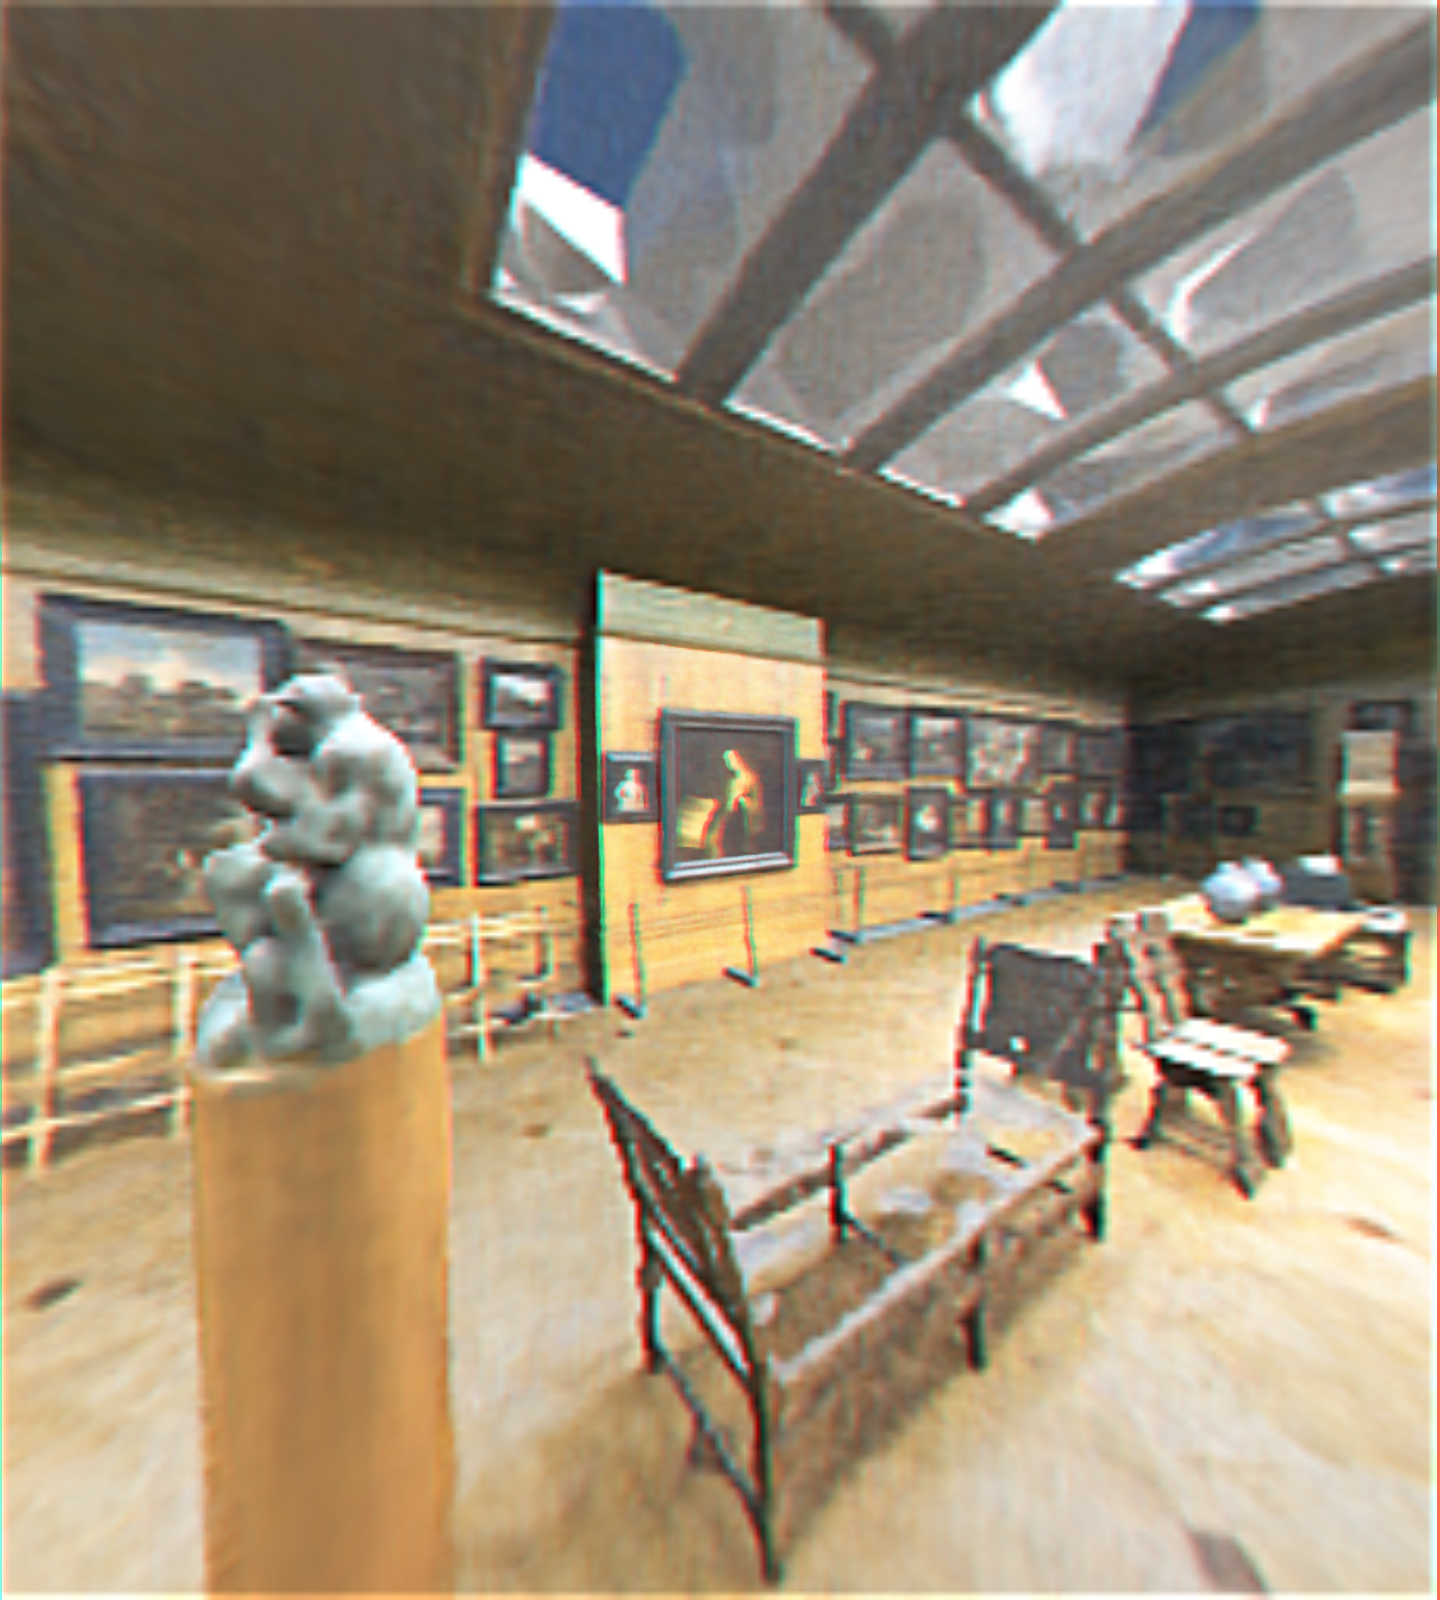
\includegraphics[width=0.248\linewidth]{TOG/figs/mono_periphery/gallery_view0000_blended_stereo.png}%\label{fig:mono:w}}
    
    \subfloat[w/o gaze-adaptive stereo]{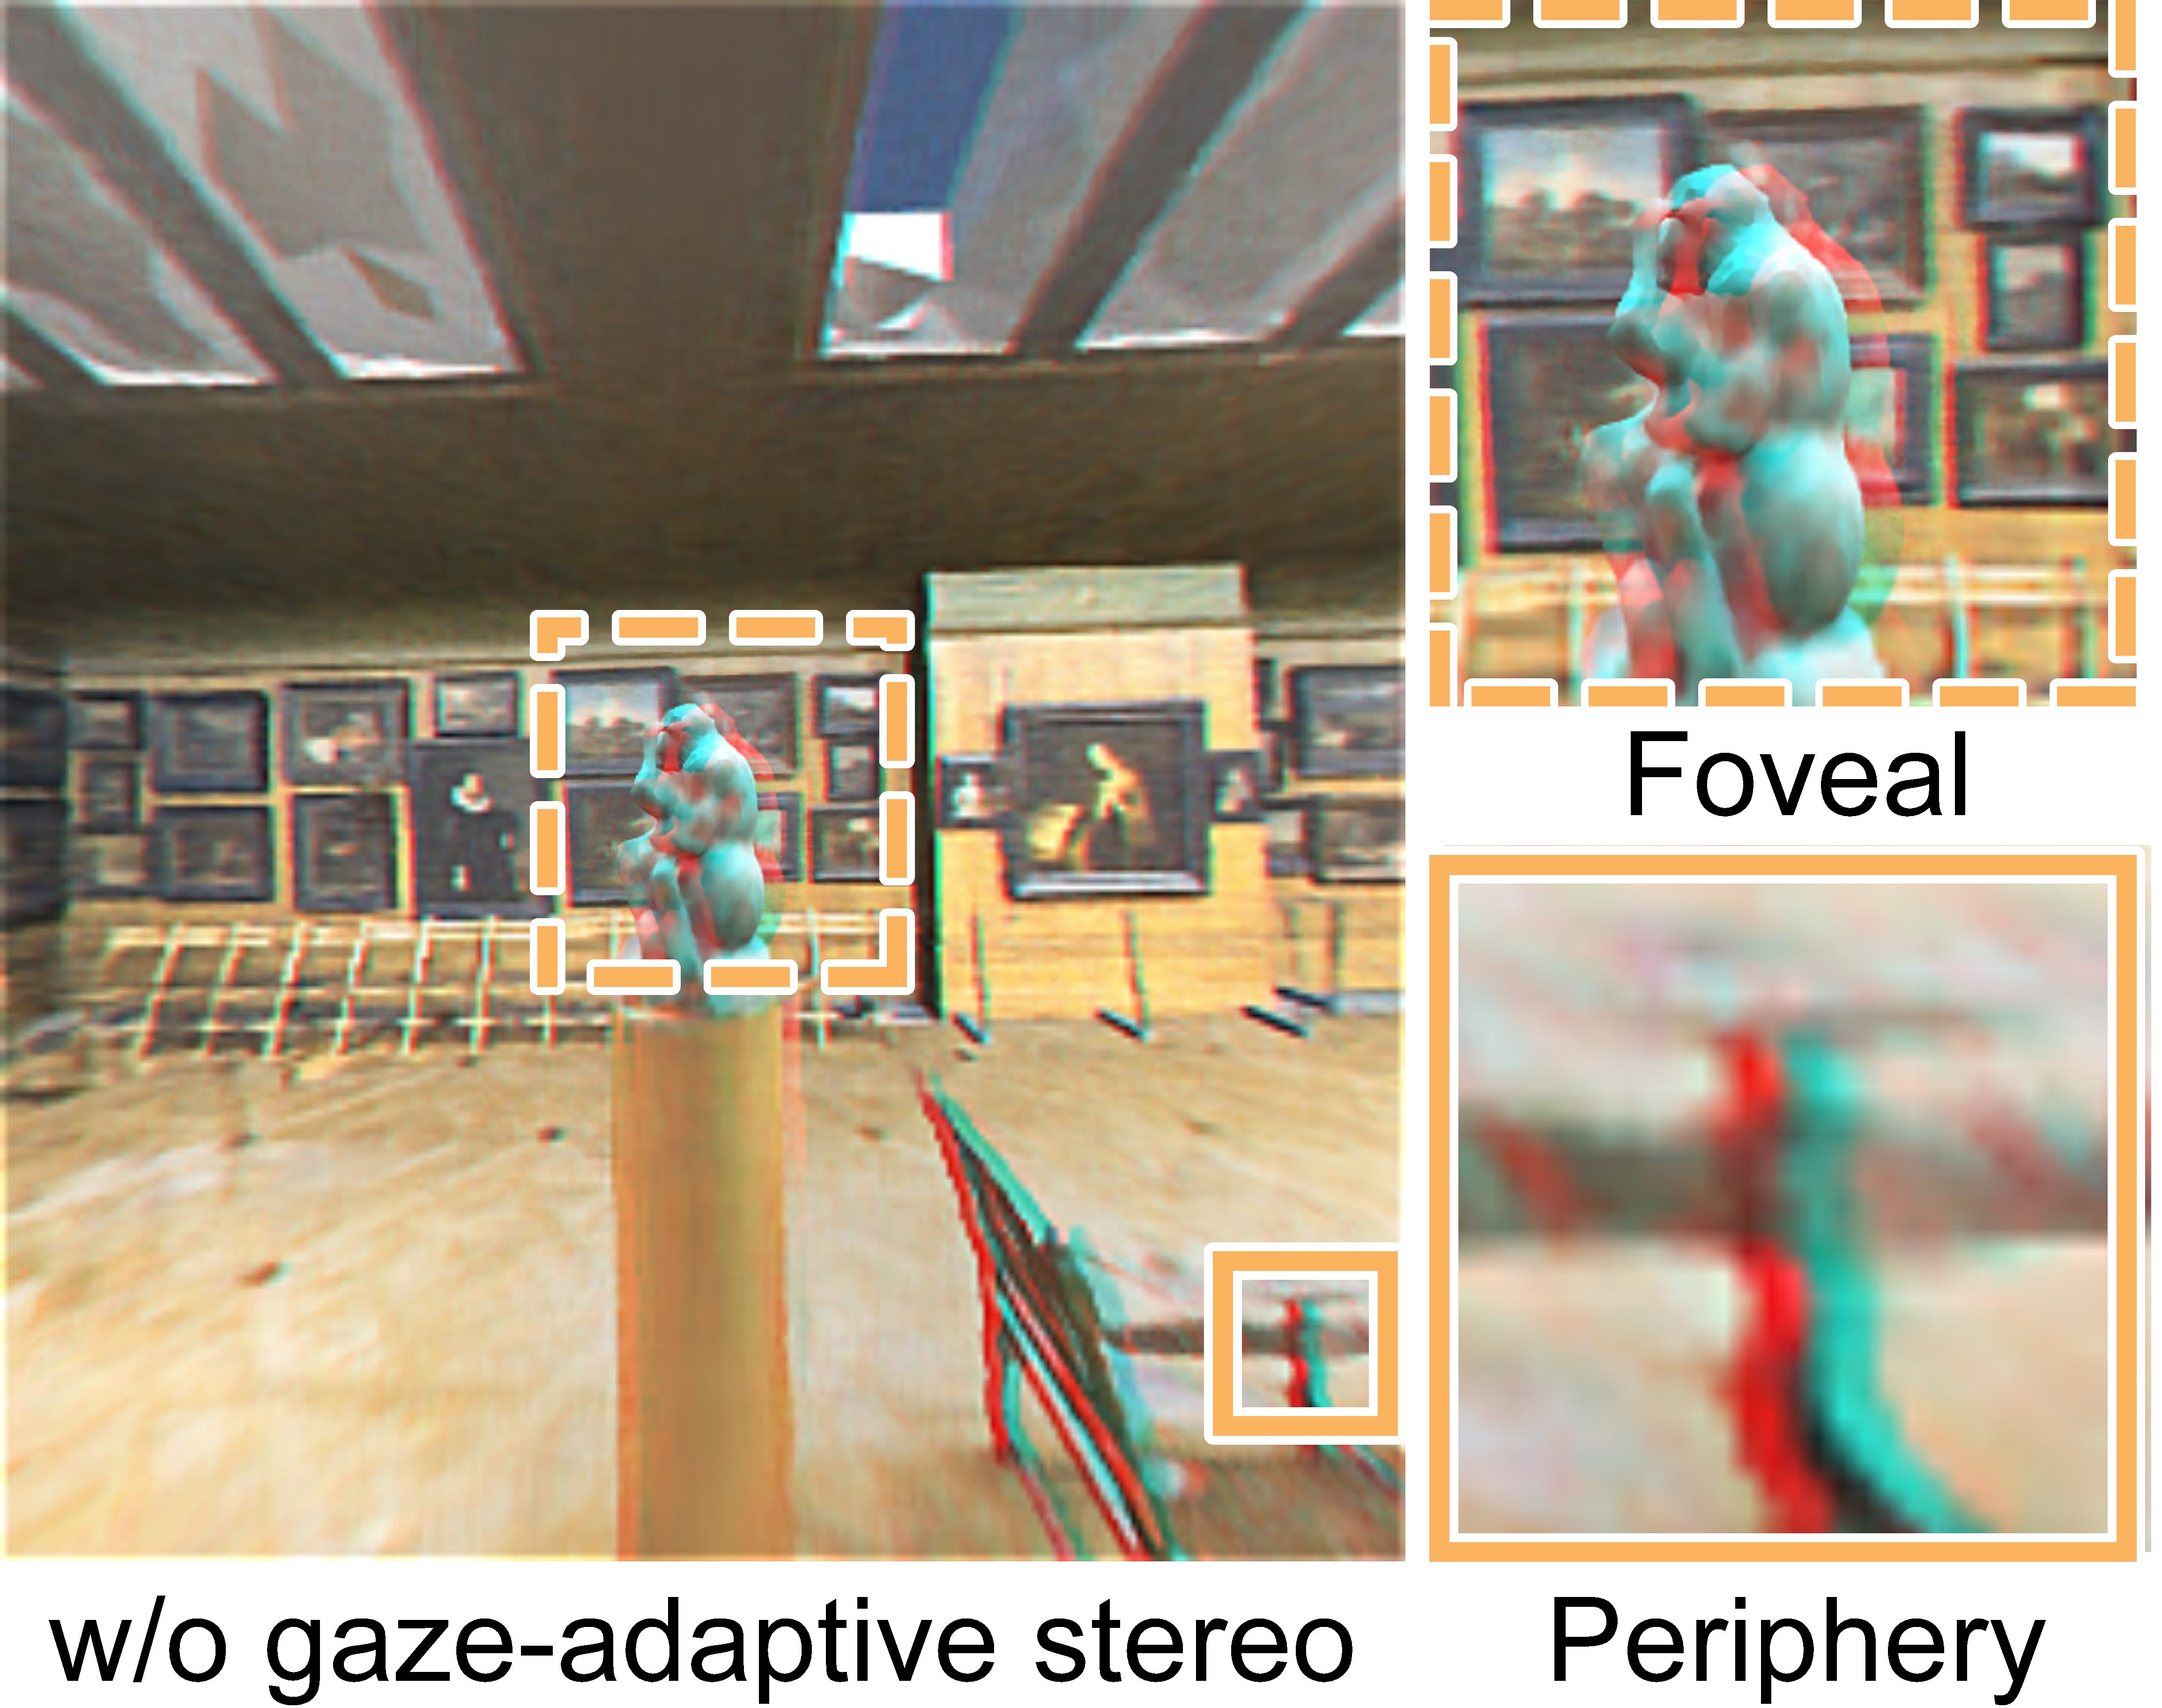
\includegraphics[width=0.48\linewidth]{TOG/figs/stereo_periphery/stereo_periphery.pdf}\label{fig:mono:wo}}%\hspace{0.5em}
    \subfloat[w/ gaze-adaptive stereo]{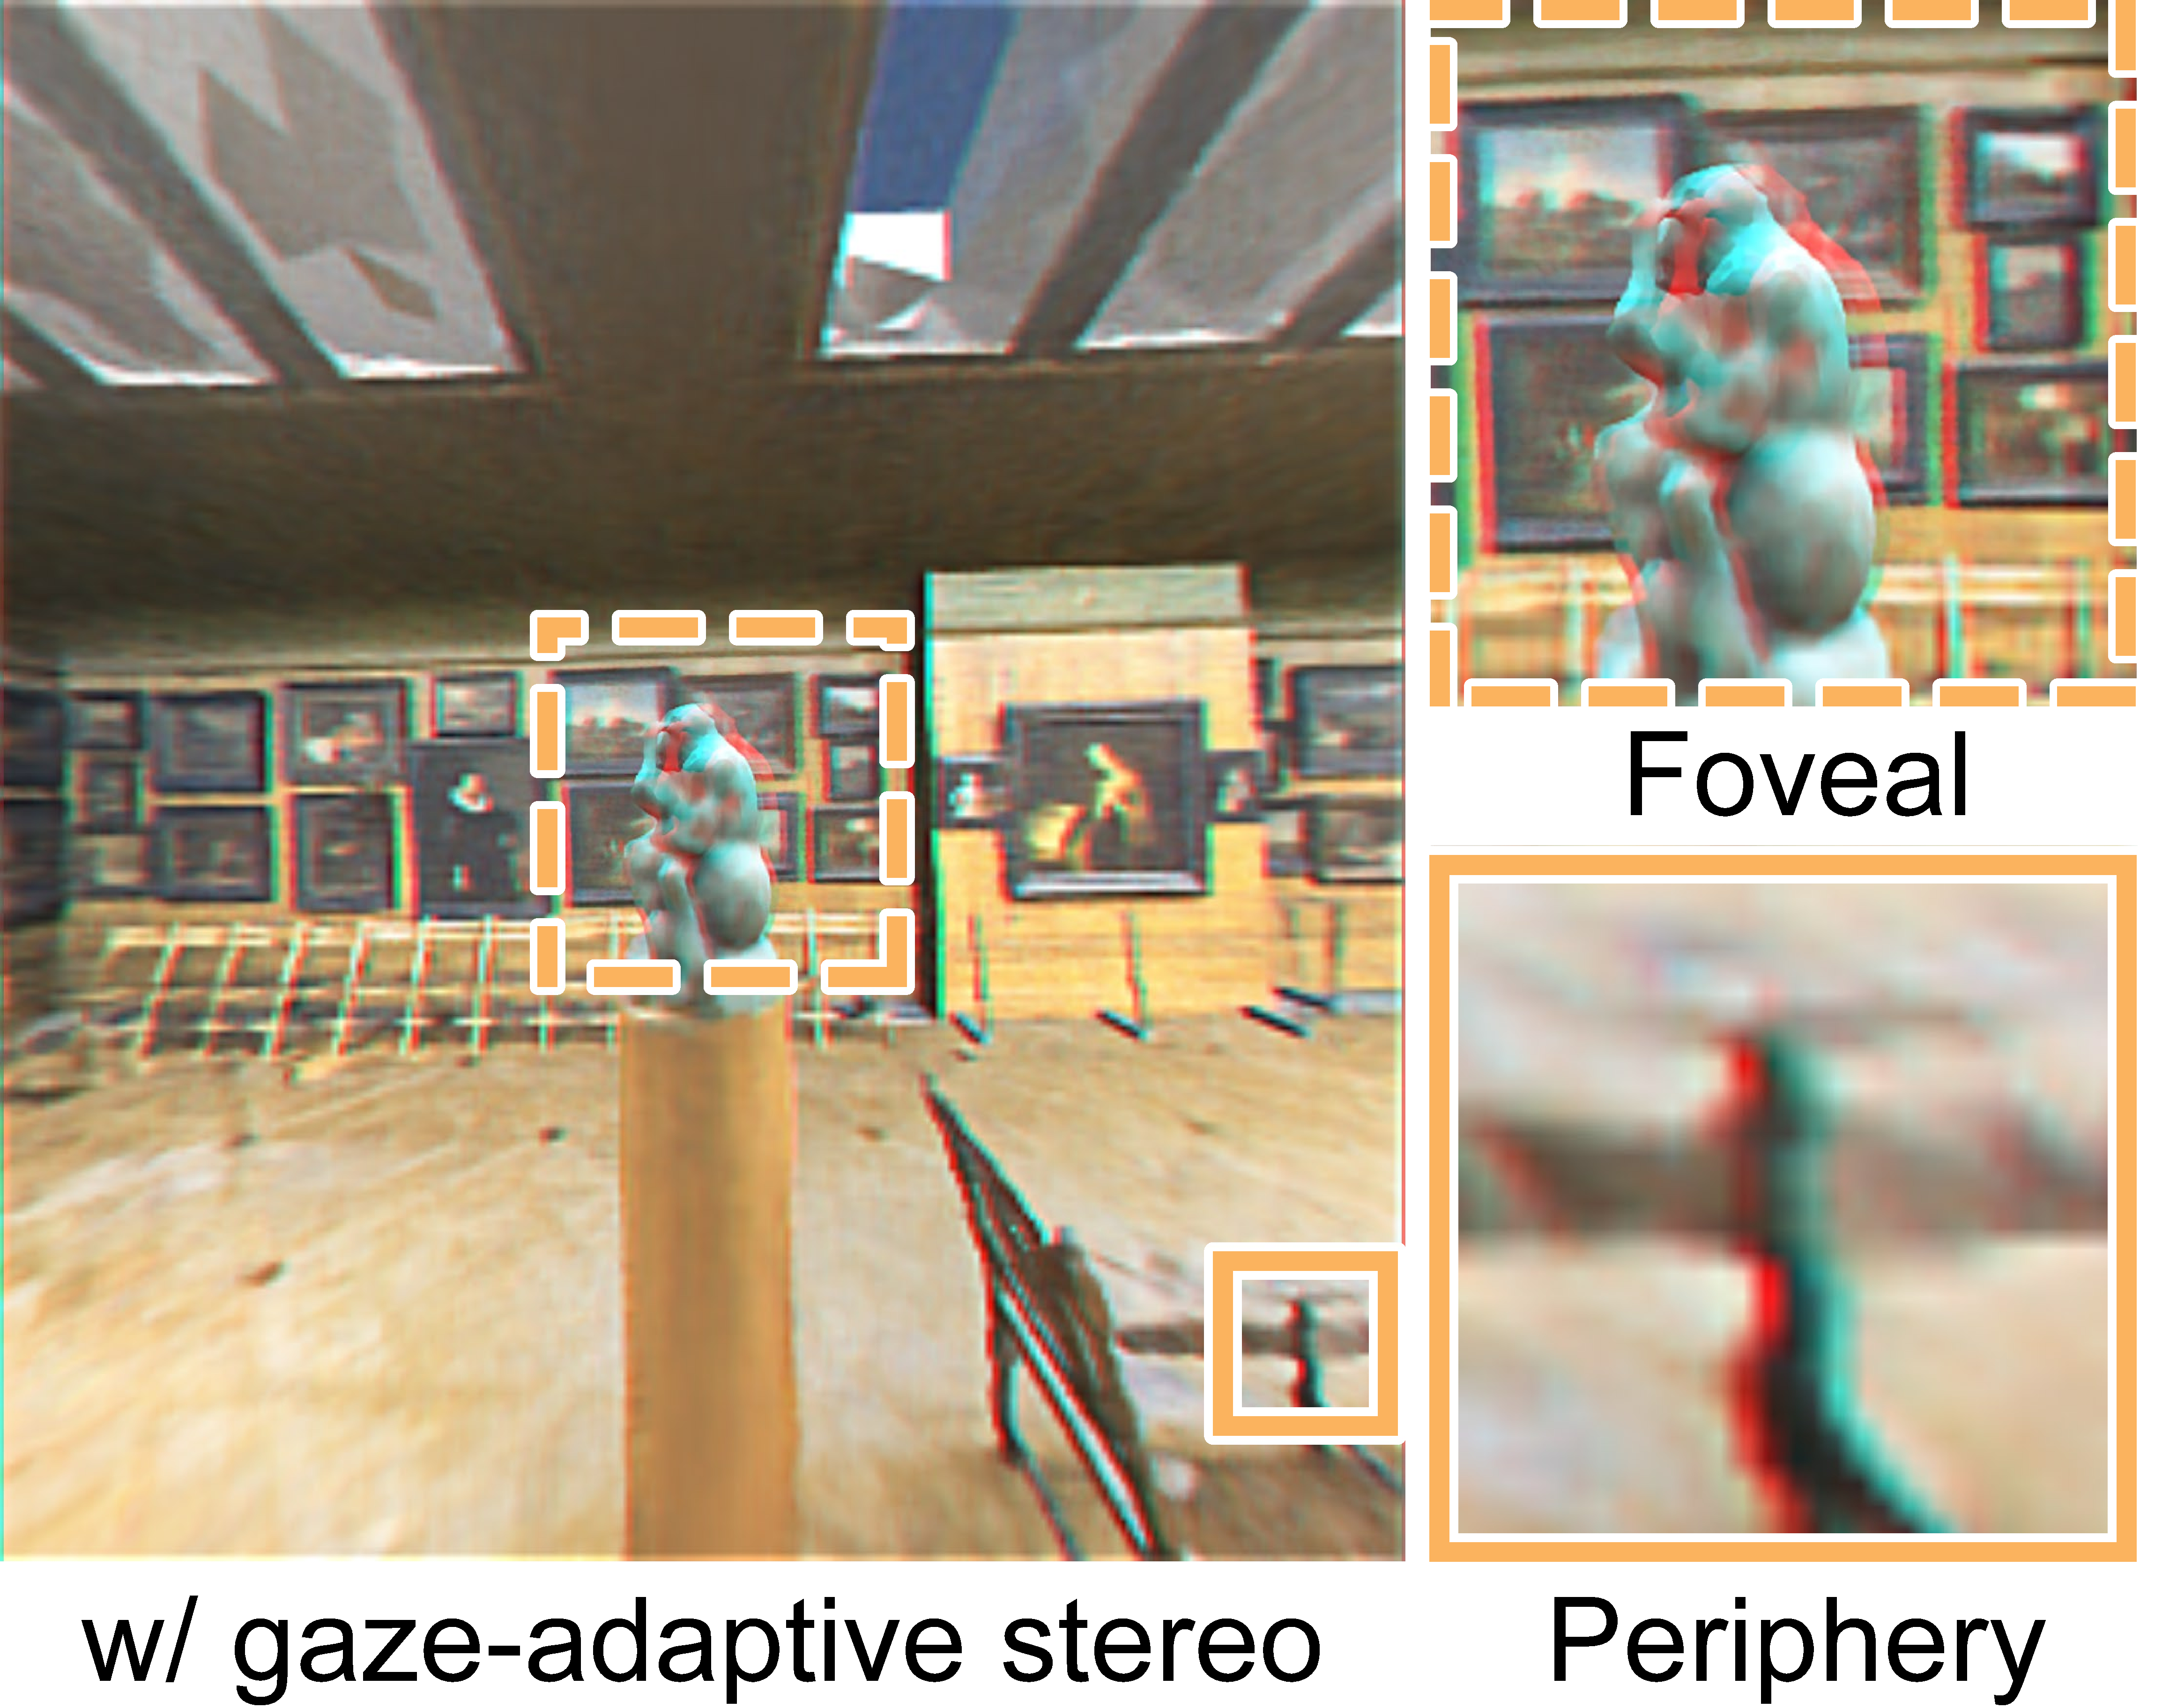
\includegraphics[width=0.48\linewidth]{TOG/figs/stereo_periphery/mono_periphery.pdf}\label{fig:mono:w}}
    %\subfloat[w/o gaze-adaptive stereo]{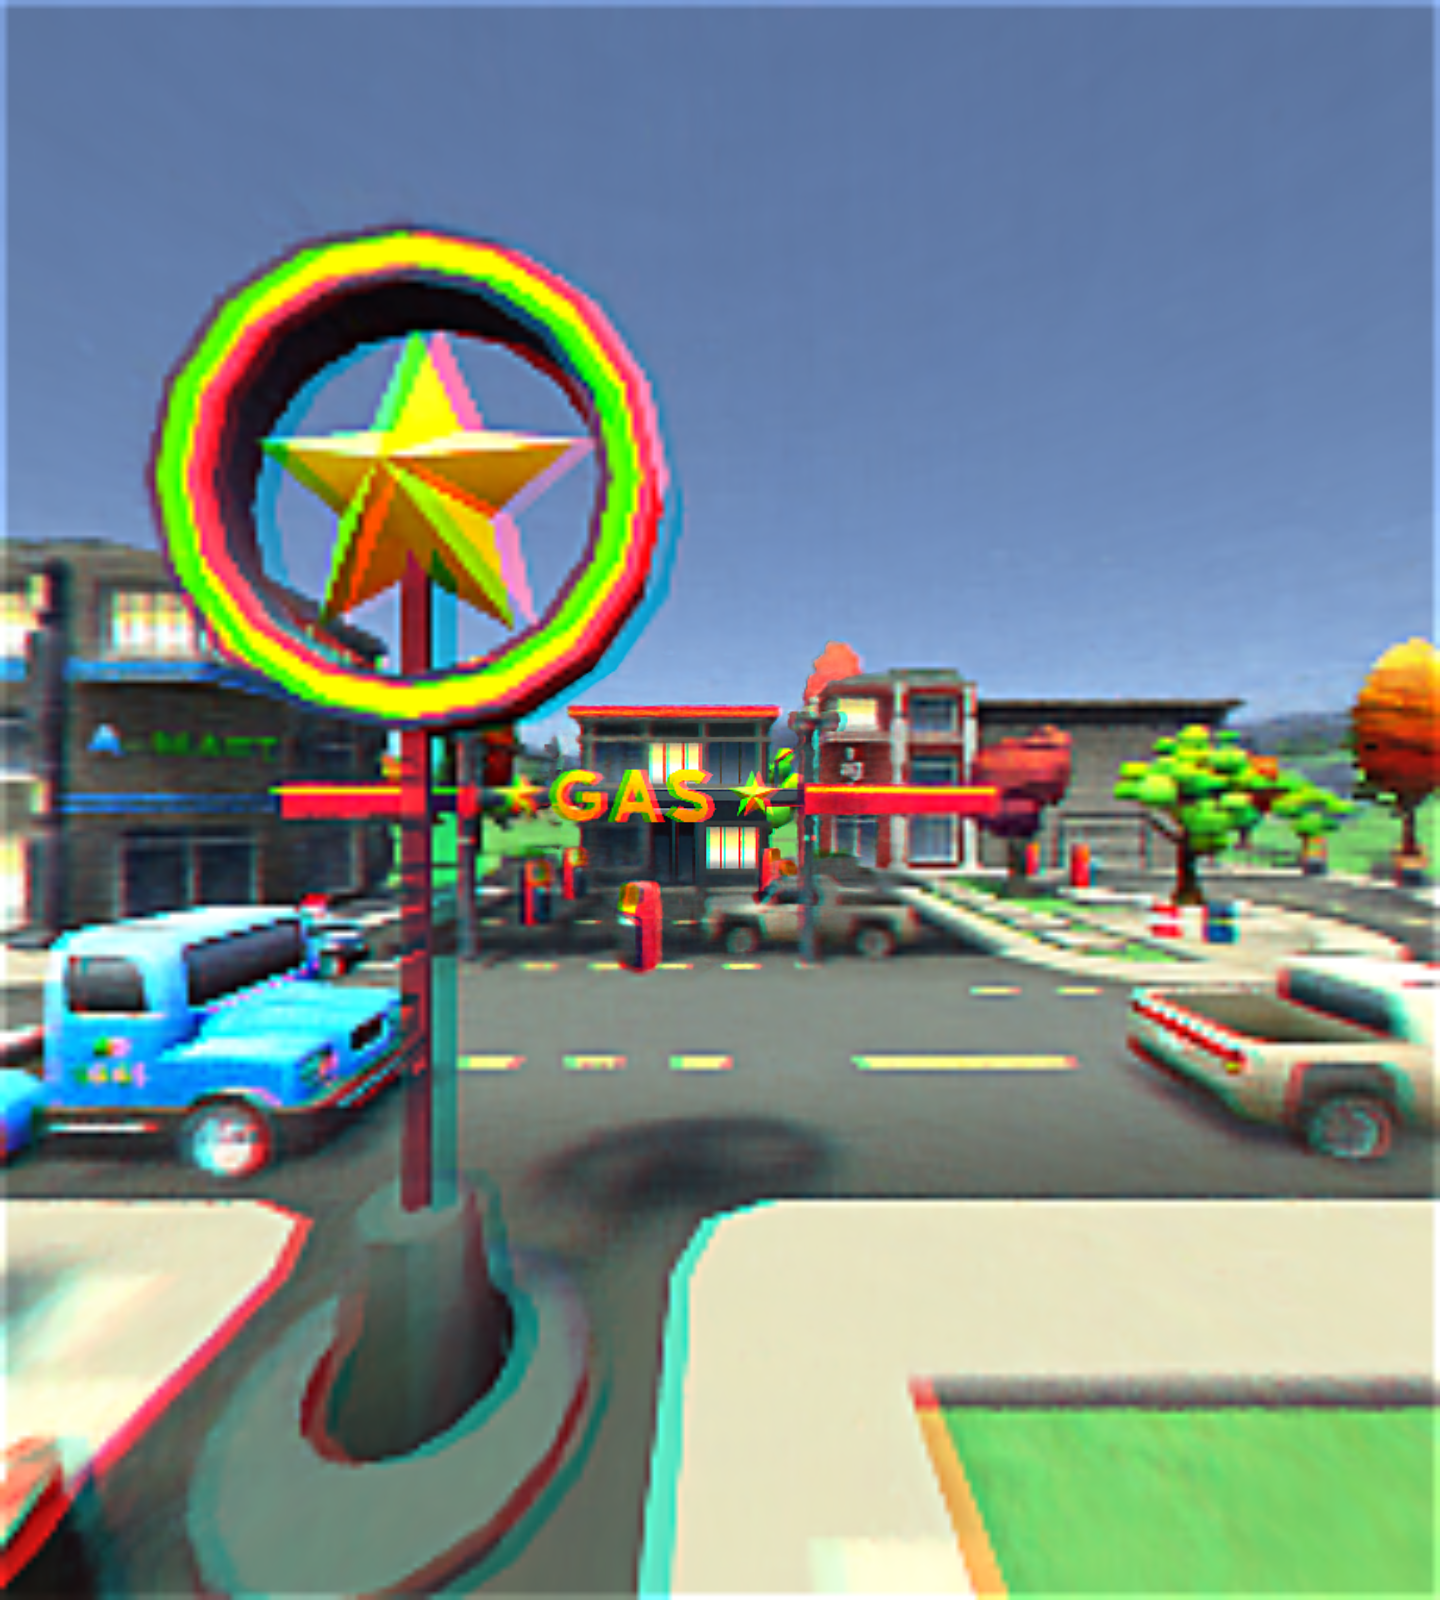
\includegraphics[width=0.248\linewidth]{TOG/figs/stereo_periphery/gas_view0000_blended_stereo.png}\label{fig:mono:wo}}
    %\subfloat[w/ gaze-adaptive stereo]{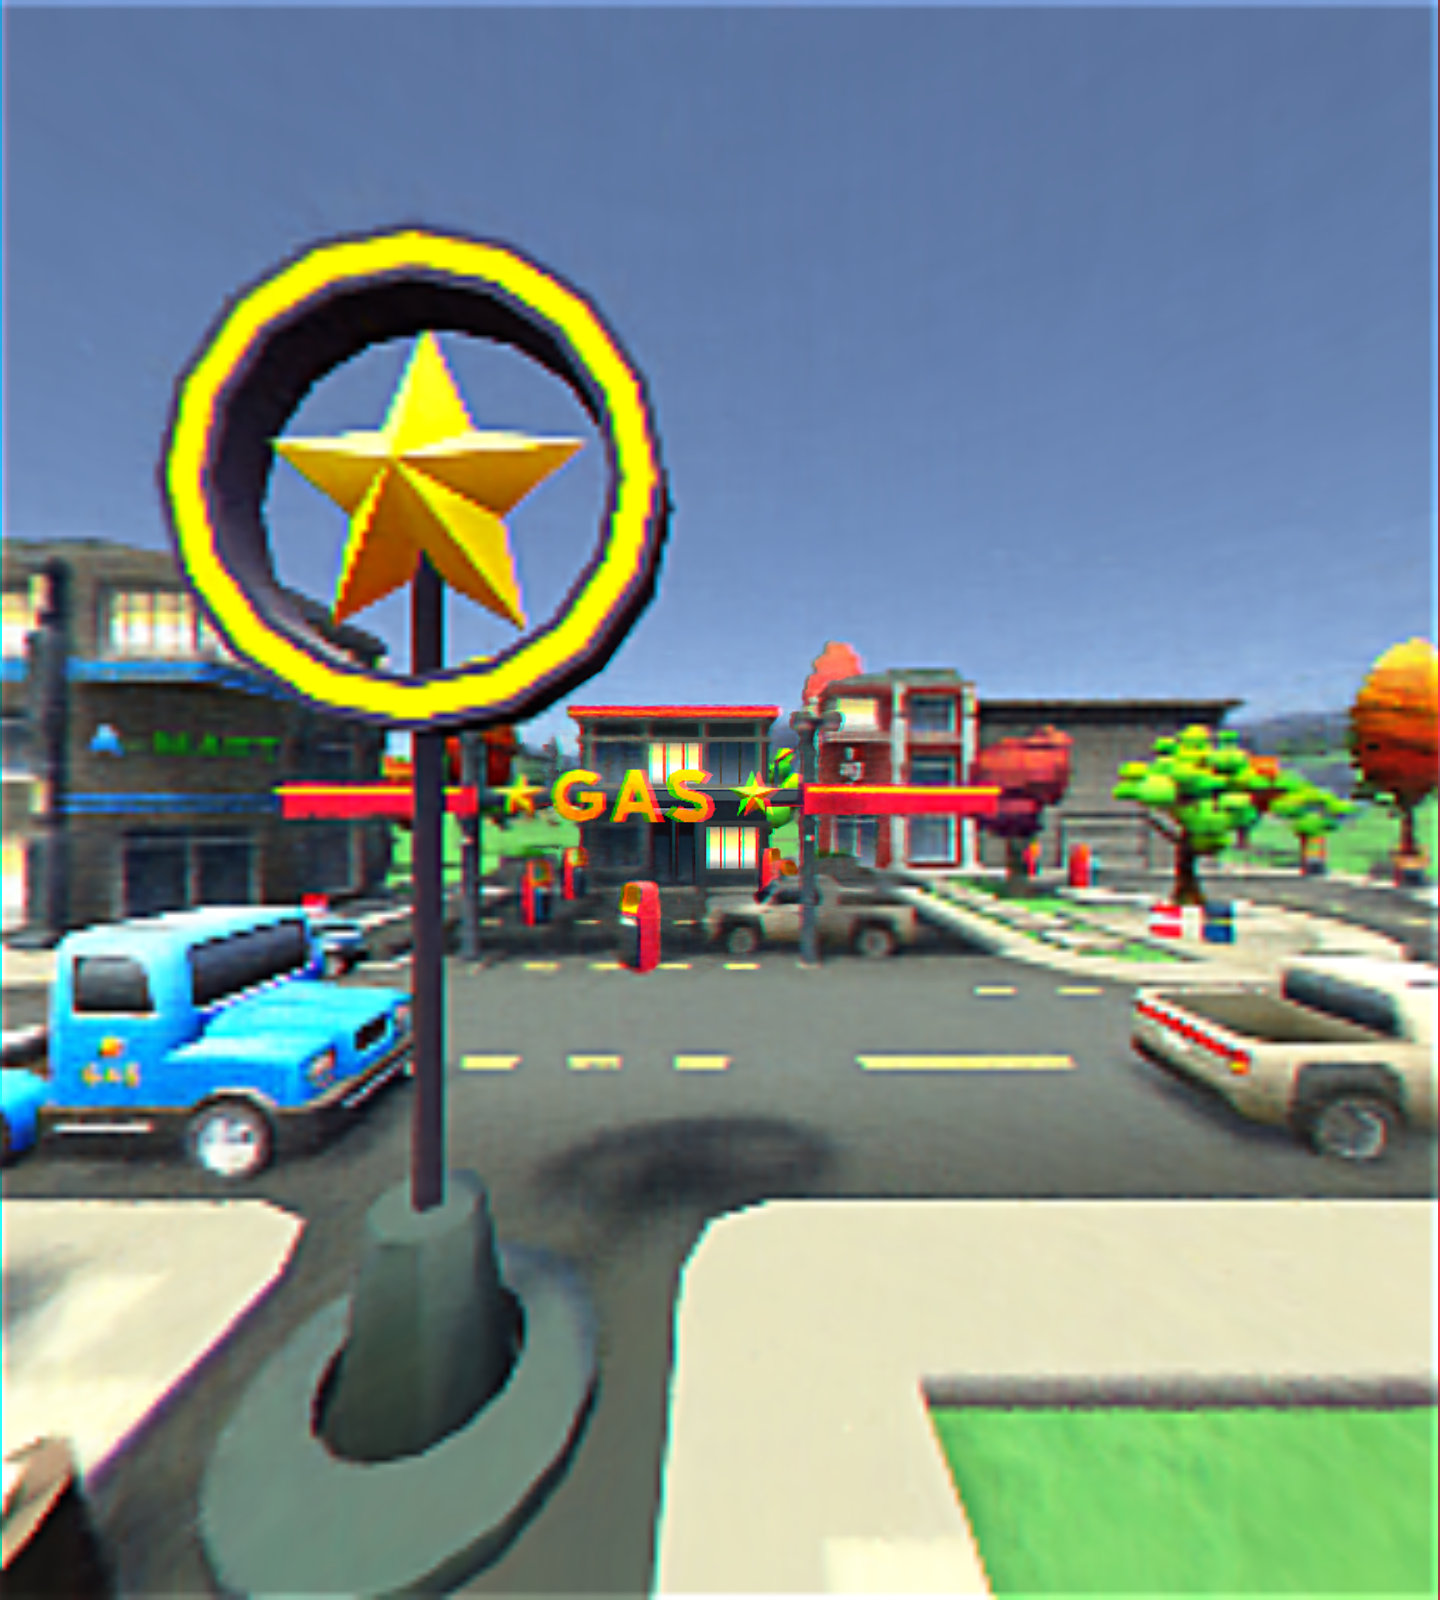
\includegraphics[width=0.248\linewidth]{TOG/figs/mono_periphery/gas_view0000_blended_stereo.png}\label{fig:mono:w}}
    
    %\subfloat[w/o gaze-adaptive stereo]{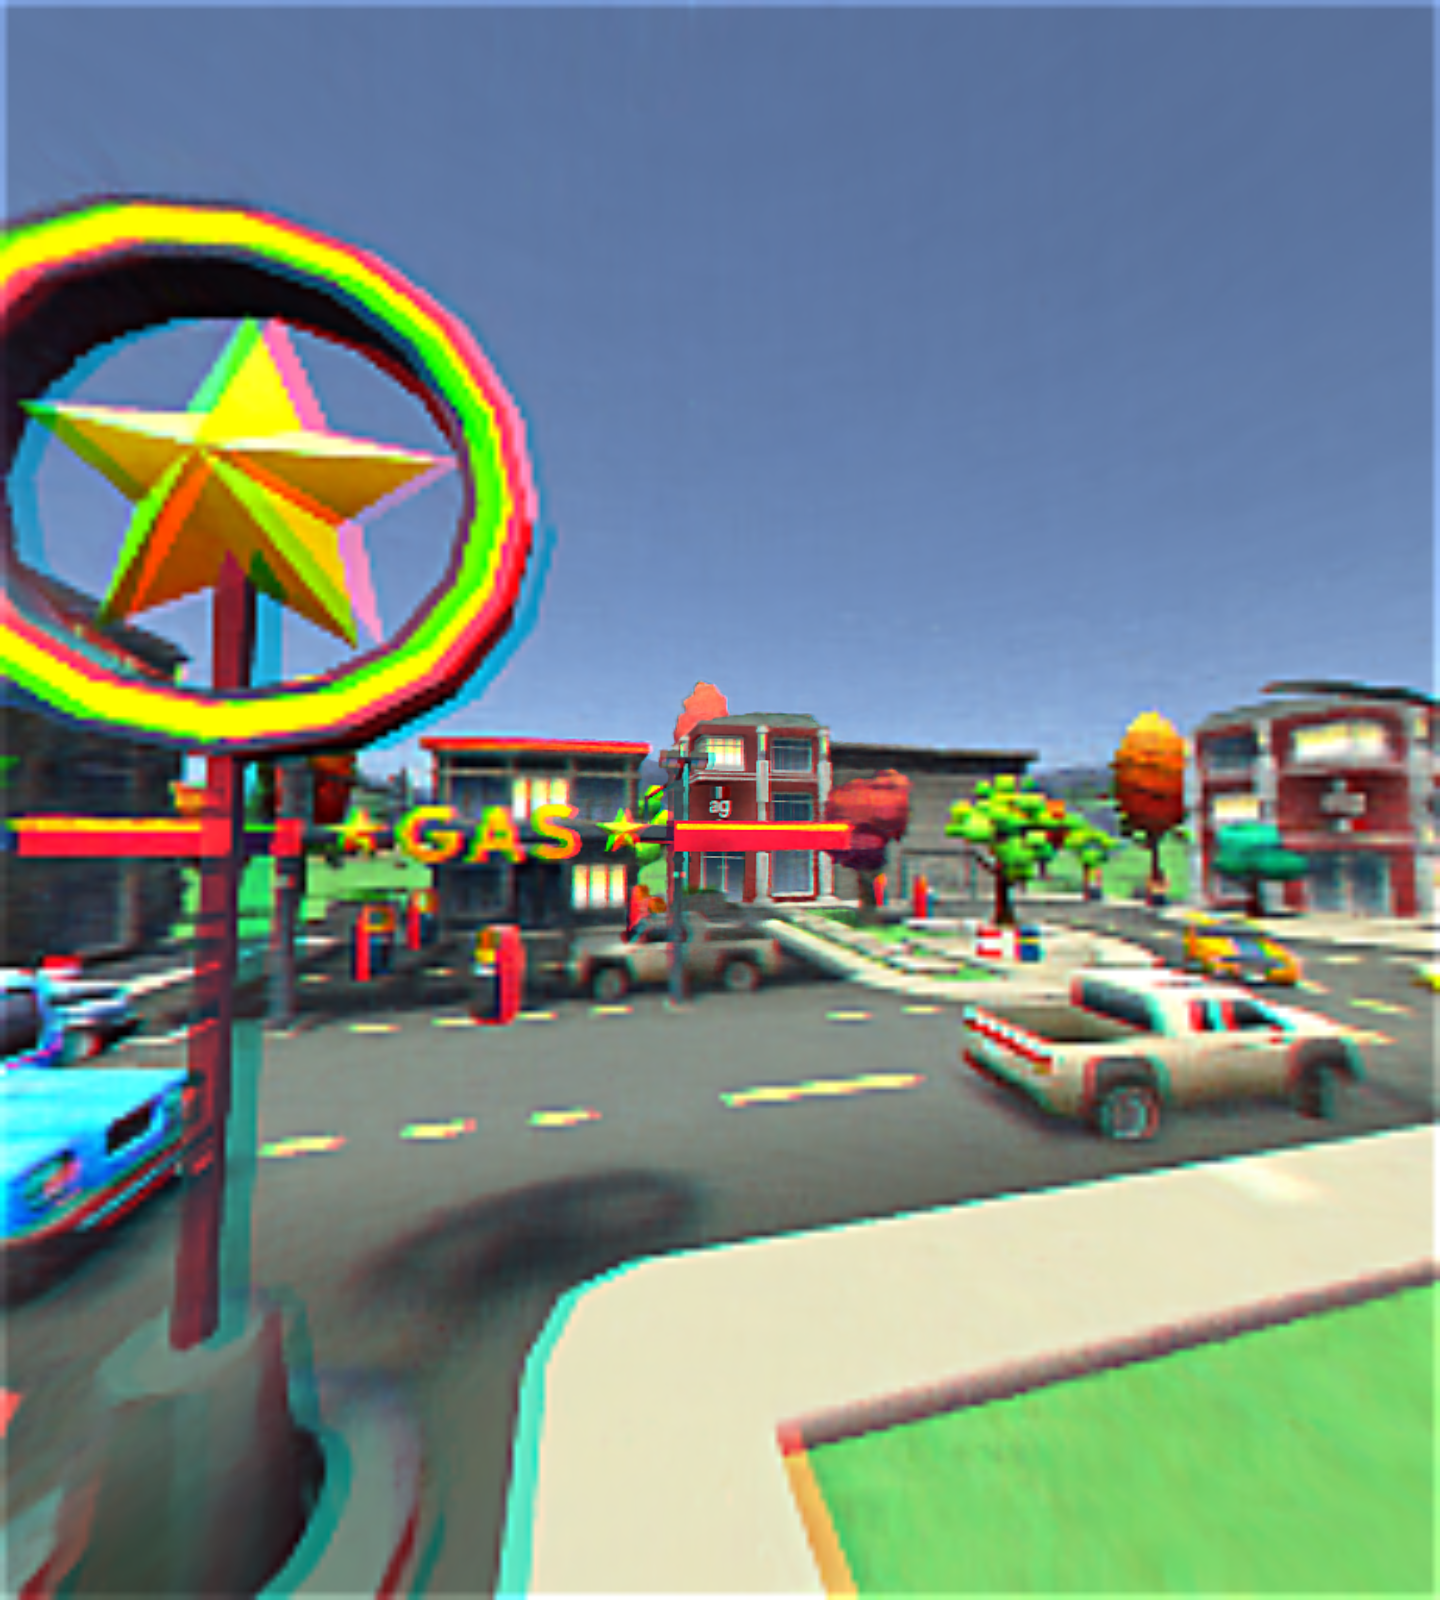
\includegraphics[width=0.248\linewidth]{TOG/figs/stereo_periphery/gas_view0001_blended_stereo.png}\label{fig:mono:wo}}
    %\subfloat[w/ gaze-adaptive stereo]{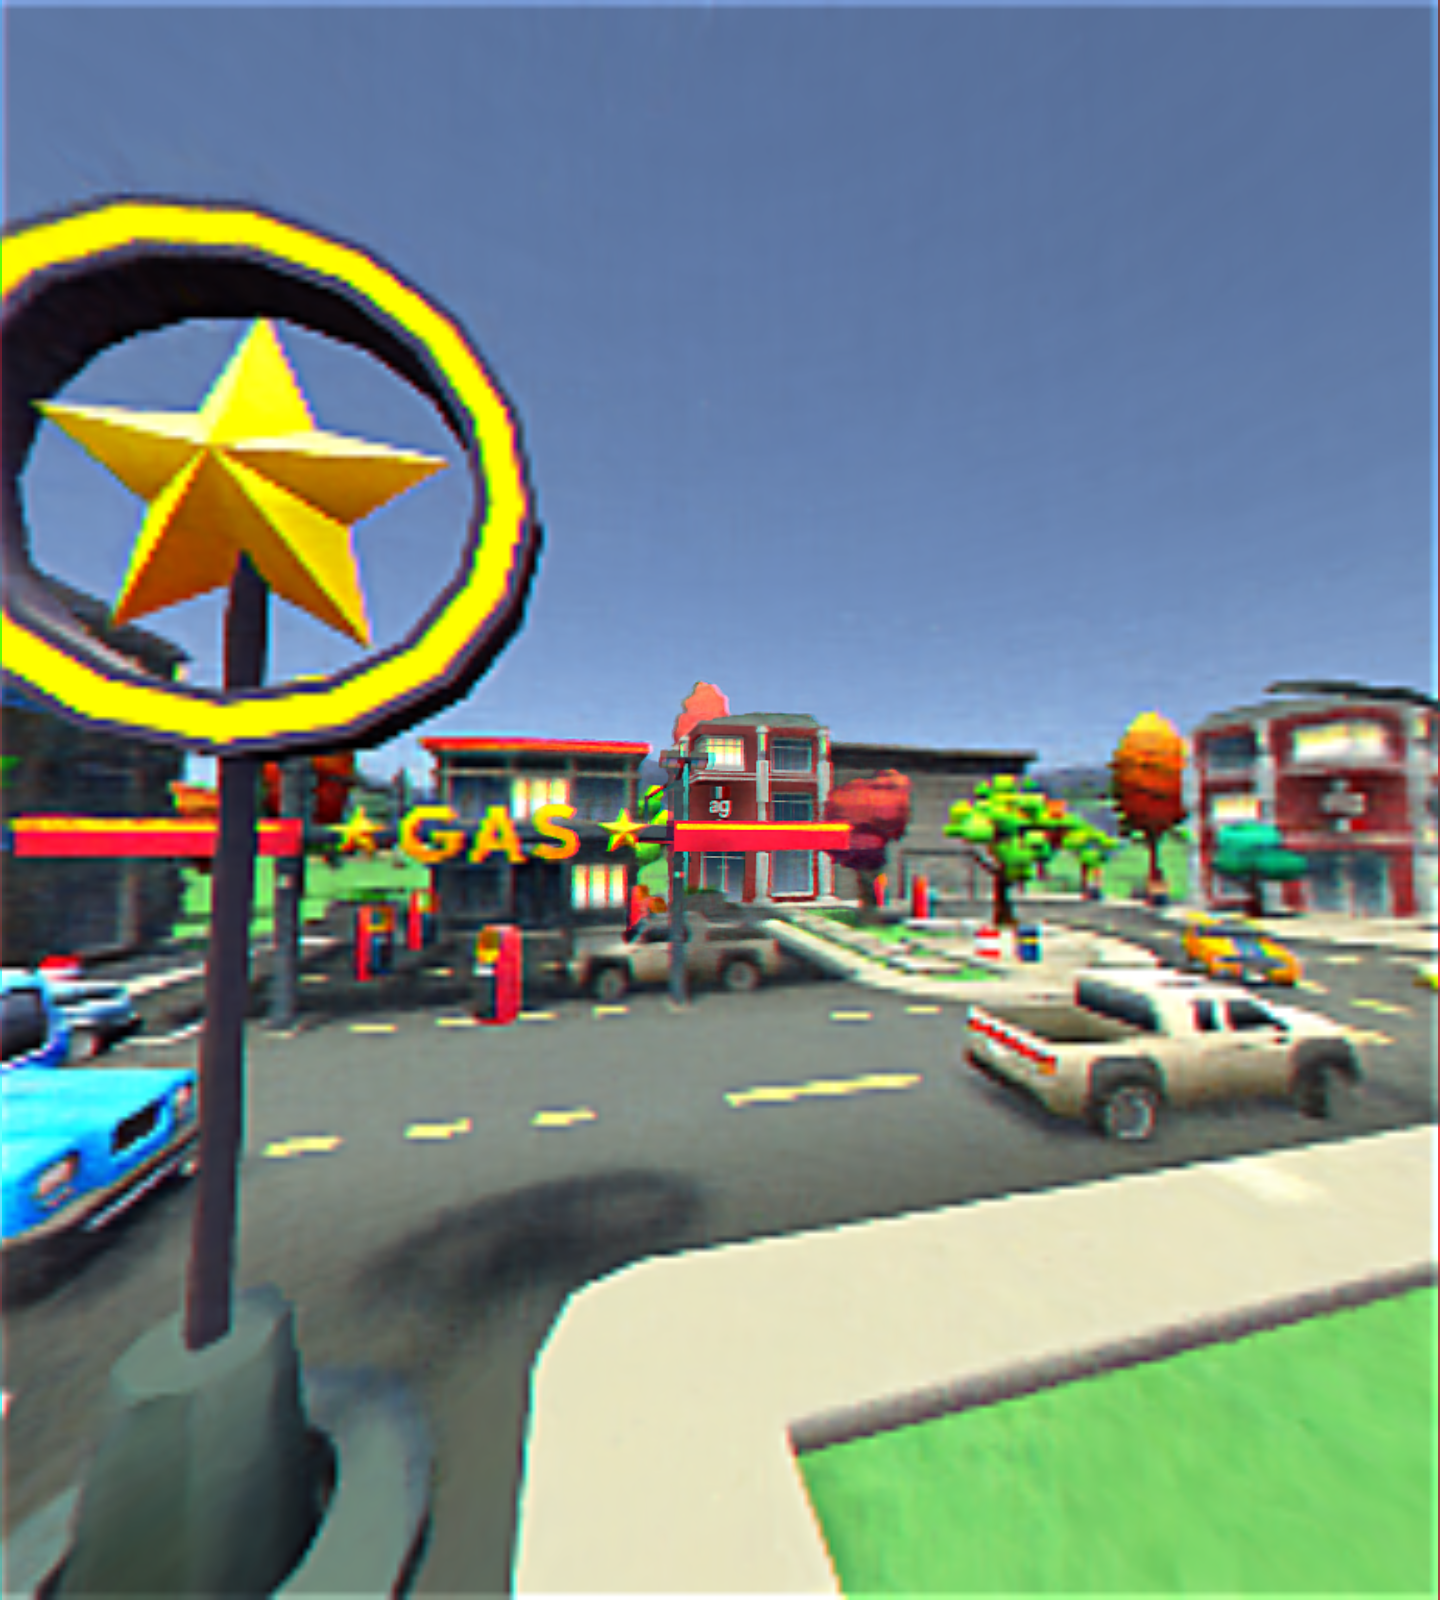
\includegraphics[width=0.248\linewidth]{TOG/figs/mono_periphery/gas_view0001_blended_stereo.png}\label{fig:mono:w}}
    \Caption{Visualization of the adaptive stereo-acuity with anaglyph.}
    {%
    \subref{fig:mono:wo} shows the rendered image with 6 retinal sub-images ($\imageFoveal^{\{l,r\}}$, $\imageMid^{\{l,r\}}$, and $\imageFar^{\{l,r\}}$).
    \subref{fig:mono:w} shows the rendered image with our adaptive and accelerated inference considering foveated stereoacuity ($\imageFoveal^{\{l,r\}}$, $\imageMid^{\{c\}}$, and $\imageFar^{\{c\}}$). Our method preserves full stereopsis in the fovea while reducing the angular resolution in the periphery for accelerated inference.
    }
    \label{fig:mono}
\end{figure}